\documentclass[10pt]{report}
\usepackage{/Users/bradenhoagland/latex/math}

\lhead{Braden Hoagland}
\chead{HW 10}
\rhead{}

\renewcommand{\theenumi}{\alph{enumi}}

\begin{document}
%\tableofcontents

{\color{blue}Problems completed: All.}

\begin{exer}[]
	$S$ generates $G$ if every element of $G$ can be written as a finite product of elements of $S \cup S^{-1}$. Suppose $\phi,\psi:G\to H$ are group homomorphisms that agree on $S$. Prove $\phi=\psi$.
\end{exer}
{\color{blue}Collaborators: None.}

Let $s^{-1} \in S^{-1}$, then since $\phi,\psi$ are homomorphisms,
\[
	\phi(s^{-1}) = \phi(s)^{-1} = \psi(s)^{-1} = \psi(s^{-1}),
\] so $\phi$ and $\psi$ agree on $S \cup S^{-1}$. Now since $S$ generates $G$, any $g \in G$ can be written $g = \prod_{i=1}^n s_{k_i}$, where the $k_i$'s index into $S \cup S^{-1}$. Then again by properties of group homomorphisms,
\[
	\phi(g) = \phi \left( \prod_{i=1}^n s_{k_i} \right) = \prod_{i=1}^n \phi(s_{k_i}) = \prod_{i=1}^n \psi(s_{k_i}) = \psi \left( \prod_{i=1}^n s_{k_i} \right) = \psi(g).
\] 
Thus $\phi = \psi$.

\pagebreak
\begin{exer}[\S 52 pg. 334 \#1]
$A \subset \mathbb{R}^{n}$ is \textbf{star convex}if there is some point $a_0$ such that all line segments joining $a_0$ to other points of $A$ lie in $A$.
\begin{enumerate}
	\item Find a star convex set that is not convex.
	\item Show that if $A$ is star convex, $A$ is simply connected.
\end{enumerate}
\end{exer}
{\color{blue}Collaborators: None.}

\begin{enumerate}
	\item Consider the set
		\begin{align*}
			A &= \left\{ (x,y) \;|\; -2 \leq x \leq 2, -1 \leq y \leq 1 \right\} \\
			&\quad \cup \left\{ (x,y) \;|\; -1 \leq x \leq 1, -2 \leq y \leq 2 \right\},
		\end{align*}
		pictured below. Every line segment from the origin to another point in $A$ lies entirely in $A$, but the line from $(1,2)$ to $(2,1)$ does not.
		\begin{figure}[H]
			\centering
			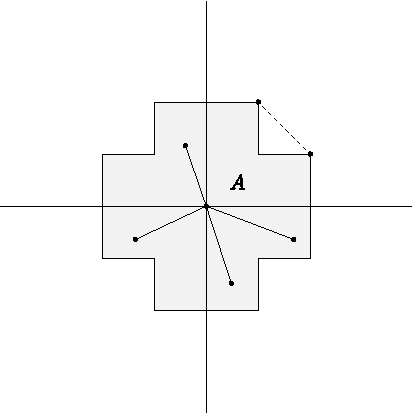
\includegraphics[scale=0.8]{fig/star.pdf}
		\end{figure}

	\item Since $A$ is star convex, for all $x,y \in A$, we can find a line segment from $a_0$ to $x$ and from $a_0$ to $y$. Pasting these two lines together gives a path form $x$ to $y$, so $A$ is path connected.

		Now suppose $f,g$ are loops based at $a_0$. Then since every point on $f,g$ has a line segment to $a_0$ lying entirely in $A$, we can use the straight line homotopy to send $f$ and $g$ to the constant map $x \mapsto a_0$. Thus $f,g \simeq_{p} x \mapsto a_0$, which implies $f \simeq_{p} g$. Since $f$ and $g$ were arbitrary, this means all loops at $a_0$ are path homotopic, so $\pi_1(A,a_0)$ is trivial.

		Since $A$ is path connected and has a trivial fundamental group at some point, $A$ is simply connected.
\end{enumerate}

\pagebreak
\begin{exer}[\S 52 pg. 335 \#5]
	If $A$ is a subspace of $\mathbb{R}^n$ and $H:(A,a_0)\to (Y,y_0)$ can be extended to a continuous map of $\mathbb{R}^n$ into $Y$, then $h_{*}$ is the trivial homomorphism.
\end{exer}
{\color{blue}Collaborators: None.}

We're given that there is some continuous $\tilde{h}:\mathbb{R}^n\to Y$ such that $h=\tilde{h} \circ i$, where $i: A \hookrightarrow \mathbb{R}^{n}$ is the usual inclusion map. Now $\mathbb{R}^n$ is simply connected, so $\pi_1(\mathbb{R}^n,a_0)$ is the trivial group. Since homomorphisms map identities to identities, the induced map $\tilde{h}_{*}$ must be the trivial homomorphism.

Since the homomorphism induced by $h$ is $h_{*} = (\tilde{h} \circ i)_{*}= \tilde{h}_{*}\circ i_{*}$, this means $h_{*}$ must also be the trivial homomorphism.

\pagebreak
\begin{exer}[\S 53 pg. 341 \#3]
	Let $p:E\to B$ be a covering map, and let $B$ be connected. Show that if $p^{-1}(b_0)$ has $k$ elements for some $b_0 \in B$, then $p^{-1}(b)$ has $k$ elemenets for all $b \in B$.
\end{exer}
{\color{blue}Collaborators: None.}

First we show that all points in any evenly covered neighbhorbood have the same number of elements in their preimage under $p$, then we use the connectedness of $B$ to make this local property global.

Fix some $\tilde{b} \in B$ and consider an evenly covered neighborhood $U$ of $\tilde{b}$. If $|p^{-1}(\tilde{b})|=k$, then we claim that $p^{-1}(U)$ has $k$ exactly homeomorphic copies of $U$. Since $p$ restricted to each $V_i \in p^{-1}(U)$ is a homeomorphism, we know that each $V_i$ maps at most 1 point to $\tilde{b}$ (one-to-one) and at least 1 point to $\tilde{b}$ (onto). Thus each $V_i$ maps exactly one point to $\tilde{b}$, so there must be $k$ such $V_i$. Then by a similar argument, any $b \in U$ is mapped to by a single point in each $V_i$, so the inverse image of any point in $U$ has $k$ elements.

We now extend this local property to all of $B$. For each $b \in B$, choose an evenly covered neighborhood $U_{b}$ of $b$. None of these neighborhoods is disjoint from all others: if there were some $U_{b'}$ disjoint from all others, then $U_{b'}, \bigcup_{b \neq b'} U_{b}$ would separate $B$, contradicting the connectedness of $B$. Thus for any $b \in B$, we can find some chain of evenly covered neighborhoods linking $U_{b}$ to $U_{b_0}$. Then all points in $U_{b}$ (in particular, the point $b$) have $k$ elements in their preimage under $p$. Thus $|p^{-1}(b)|=k$ for all $b \in B$.

\pagebreak
\begin{exer}[]
	Suppose $f,g:X\to S^2 = \left\{ (x,y,z) \;|\; z^2+y^2+z^2=1 \right\}$ satisfy $f(x) \neq -g(x)$ for all $x \in X$. Prove that $f$ and $g$ are homotopic.
\end{exer}
{\color{blue}Collaborators: None.}

Let $F(x,t) = (1-t)f(x) + tg(x)$. This is the form of the usual straight line homotopy, but it doesn't work in our case since it doesn't lie entirely in $S^2$; however, we can modify it to remain on $S^2$ by
\[
	\tilde{F}(x,t) = \frac{F(x,t)}{{\Vert{F(x,t)}\Vert}} .
\] Since $f(x)$ and $g(x)$ are assumed to never be antipodal, we know that $F(x,t)$ never crosses the origin. This means ${\Vert{F(x,t)}\Vert}$ is never 0, so $\tilde{F}$ is well-defined. It has norm ${\Vert{\tilde{F}(x,t)}\Vert}=1$, and since we've defined $S^2$ to be all points in $\mathbb{R}^3$ with norm 1, $\tilde{F}$ lies entirely in $S^2$. Thus $\tilde{F}$ is a homotopy from $f$ to $g$.

\end{document}
